% Created by tikzDevice version 0.12.3.1 on 2022-09-01 15:55:02
% !TEX encoding = UTF-8 Unicode
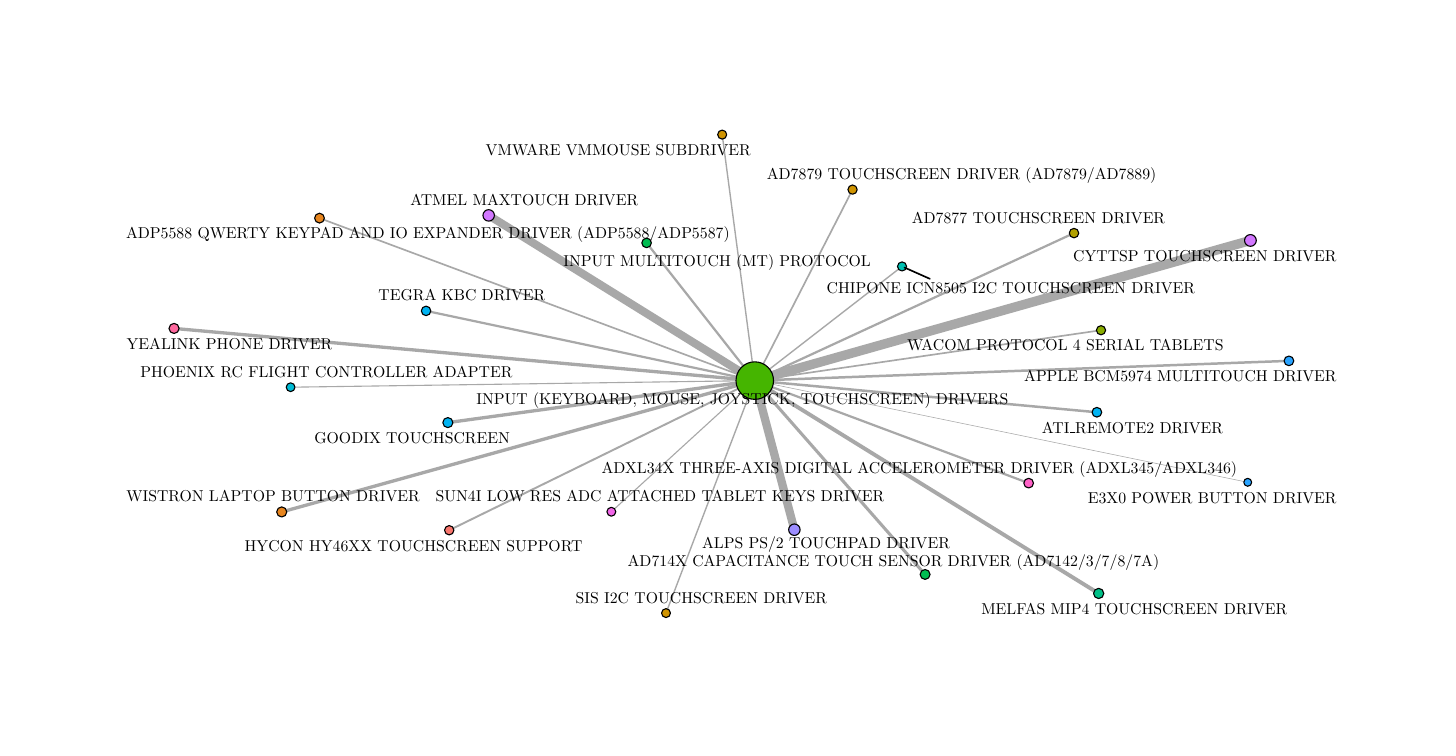
\begin{tikzpicture}[x=1pt,y=1pt]
\definecolor{fillColor}{RGB}{255,255,255}
\path[use as bounding box,fill=fillColor,fill opacity=0.00] (0,0) rectangle (505.89,252.94);
\begin{scope}
\path[clip] (  0.00,  0.00) rectangle (505.89,252.94);
\definecolor{fillColor}{RGB}{255,255,255}

\path[fill=fillColor] (  0.00,  0.00) rectangle (505.89,252.94);
\end{scope}
\begin{scope}
\path[clip] ( 32.75, 32.75) rectangle (475.89,222.94);
\definecolor{drawColor}{gray}{0.66}

\path[draw=drawColor,line width= 1.1pt,line join=round] (324.28, 55.36) -- (262.73,125.41);

\path[draw=drawColor,line width= 0.8pt,line join=round] (378.09,178.71) -- (262.73,125.41);

\path[draw=drawColor,line width= 0.6pt,line join=round] (298.07,194.42) -- (262.73,125.41);

\path[draw=drawColor,line width= 0.6pt,line join=round] (105.45,184.12) -- (262.73,125.41);

\path[draw=drawColor,line width= 0.8pt,line join=round] (361.70, 88.36) -- (262.73,125.41);

\path[draw=drawColor,line width= 3.0pt,line join=round] (277.05, 71.53) -- (262.73,125.41);

\path[draw=drawColor,line width= 0.9pt,line join=round] (455.75,132.54) -- (262.73,125.41);

\path[draw=drawColor,line width= 0.9pt,line join=round] (386.36,113.97) -- (262.73,125.41);

\path[draw=drawColor,line width= 2.9pt,line join=round] (166.58,185.11) -- (262.73,125.41);

\path[draw=drawColor,line width= 0.5pt,line join=round] (315.95,166.66) -- (262.73,125.41);

\path[draw=drawColor,line width= 3.4pt,line join=round] (441.84,176.05) -- (262.73,125.41);

\path[draw=drawColor,line width= 0.2pt,line join=round] (440.86, 88.66) -- (262.73,125.41);

\path[draw=drawColor,line width= 1.2pt,line join=round] (151.83,110.23) -- (262.73,125.41);

\path[draw=drawColor,line width= 0.7pt,line join=round] (152.32, 71.34) -- (262.73,125.41);

\path[draw=drawColor,line width= 0.8pt,line join=round] (262.73,125.41) -- (223.65,175.17);

\path[draw=drawColor,line width= 1.4pt,line join=round] (262.73,125.41) -- (387.00, 48.50);

\path[draw=drawColor,line width= 0.4pt,line join=round] (262.73,125.41) -- ( 95.01,123.02);

\path[draw=drawColor,line width= 0.5pt,line join=round] (262.73,125.41) -- (230.66, 41.40);

\path[draw=drawColor,line width= 0.4pt,line join=round] (262.73,125.41) -- (210.91, 78.02);

\path[draw=drawColor,line width= 0.8pt,line join=round] (262.73,125.41) -- (143.96,150.60);

\path[draw=drawColor,line width= 0.5pt,line join=round] (262.73,125.41) -- (250.96,214.30);

\path[draw=drawColor,line width= 0.6pt,line join=round] (262.73,125.41) -- (387.85,143.61);

\path[draw=drawColor,line width= 1.2pt,line join=round] (262.73,125.41) -- ( 91.80, 77.95);

\path[draw=drawColor,line width= 1.2pt,line join=round] (262.73,125.41) -- ( 52.89,144.26);
\definecolor{drawColor}{RGB}{0,0,0}
\definecolor{fillColor}{RGB}{0,188,81}

\path[draw=drawColor,line width= 0.4pt,line join=round,line cap=round,fill=fillColor] (324.28, 55.36) circle (  1.79);
\definecolor{fillColor}{RGB}{178,161,0}

\path[draw=drawColor,line width= 0.4pt,line join=round,line cap=round,fill=fillColor] (378.09,178.71) circle (  1.71);
\definecolor{fillColor}{RGB}{208,148,0}

\path[draw=drawColor,line width= 0.4pt,line join=round,line cap=round,fill=fillColor] (298.07,194.42) circle (  1.67);
\definecolor{fillColor}{RGB}{231,133,30}

\path[draw=drawColor,line width= 0.4pt,line join=round,line cap=round,fill=fillColor] (105.45,184.12) circle (  1.77);
\definecolor{fillColor}{RGB}{255,97,199}

\path[draw=drawColor,line width= 0.4pt,line join=round,line cap=round,fill=fillColor] (361.70, 88.36) circle (  1.75);
\definecolor{fillColor}{RGB}{156,141,255}

\path[draw=drawColor,line width= 0.4pt,line join=round,line cap=round,fill=fillColor] (277.05, 71.53) circle (  2.07);
\definecolor{fillColor}{RGB}{41,163,255}

\path[draw=drawColor,line width= 0.4pt,line join=round,line cap=round,fill=fillColor] (455.75,132.54) circle (  1.75);
\definecolor{fillColor}{RGB}{0,179,242}

\path[draw=drawColor,line width= 0.4pt,line join=round,line cap=round,fill=fillColor] (386.36,113.97) circle (  1.75);
\definecolor{fillColor}{RGB}{210,119,255}

\path[draw=drawColor,line width= 0.4pt,line join=round,line cap=round,fill=fillColor] (166.58,185.11) circle (  2.07);
\definecolor{fillColor}{RGB}{0,192,178}

\path[draw=drawColor,line width= 0.4pt,line join=round,line cap=round,fill=fillColor] (315.95,166.66) circle (  1.64);
\definecolor{fillColor}{RGB}{210,119,255}

\path[draw=drawColor,line width= 0.4pt,line join=round,line cap=round,fill=fillColor] (441.84,176.05) circle (  2.12);
\definecolor{fillColor}{RGB}{41,163,255}

\path[draw=drawColor,line width= 0.4pt,line join=round,line cap=round,fill=fillColor] (440.86, 88.66) circle (  1.43);
\definecolor{fillColor}{RGB}{0,179,242}

\path[draw=drawColor,line width= 0.4pt,line join=round,line cap=round,fill=fillColor] (151.83,110.23) circle (  1.82);
\definecolor{fillColor}{RGB}{248,118,109}

\path[draw=drawColor,line width= 0.4pt,line join=round,line cap=round,fill=fillColor] (152.32, 71.34) circle (  1.69);
\definecolor{fillColor}{RGB}{69,181,0}

\path[draw=drawColor,line width= 0.4pt,line join=round,line cap=round,fill=fillColor] (262.73,125.41) circle (  6.78);
\definecolor{fillColor}{RGB}{0,188,81}

\path[draw=drawColor,line width= 0.4pt,line join=round,line cap=round,fill=fillColor] (223.65,175.17) circle (  1.73);
\definecolor{fillColor}{RGB}{0,192,135}

\path[draw=drawColor,line width= 0.4pt,line join=round,line cap=round,fill=fillColor] (387.00, 48.50) circle (  1.85);
\definecolor{fillColor}{RGB}{0,188,214}

\path[draw=drawColor,line width= 0.4pt,line join=round,line cap=round,fill=fillColor] ( 95.01,123.02) circle (  1.58);
\definecolor{fillColor}{RGB}{208,148,0}

\path[draw=drawColor,line width= 0.4pt,line join=round,line cap=round,fill=fillColor] (230.66, 41.40) circle (  1.61);
\definecolor{fillColor}{RGB}{241,102,232}

\path[draw=drawColor,line width= 0.4pt,line join=round,line cap=round,fill=fillColor] (210.91, 78.02) circle (  1.60);
\definecolor{fillColor}{RGB}{0,179,242}

\path[draw=drawColor,line width= 0.4pt,line join=round,line cap=round,fill=fillColor] (143.96,150.60) circle (  1.71);
\definecolor{fillColor}{RGB}{208,148,0}

\path[draw=drawColor,line width= 0.4pt,line join=round,line cap=round,fill=fillColor] (250.96,214.30) circle (  1.63);
\definecolor{fillColor}{RGB}{137,172,0}

\path[draw=drawColor,line width= 0.4pt,line join=round,line cap=round,fill=fillColor] (387.85,143.61) circle (  1.66);
\definecolor{fillColor}{RGB}{231,133,30}

\path[draw=drawColor,line width= 0.4pt,line join=round,line cap=round,fill=fillColor] ( 91.80, 77.95) circle (  1.82);
\definecolor{fillColor}{RGB}{255,104,158}

\path[draw=drawColor,line width= 0.4pt,line join=round,line cap=round,fill=fillColor] ( 52.89,144.26) circle (  1.82);

\path[draw=drawColor,line width= 0.6pt,line join=round,line cap=round] (326.01,162.19) -- (316.83,166.27);

\node[text=drawColor,anchor=base,inner sep=0pt, outer sep=0pt, scale=  0.57] at (312.83, 58.29) {AD714X CAPACITANCE TOUCH SENSOR DRIVER (AD7142/3/7/8/7A)};

\node[text=drawColor,anchor=base,inner sep=0pt, outer sep=0pt, scale=  0.57] at (365.25,182.28) {AD7877 TOUCHSCREEN DRIVER};

\node[text=drawColor,anchor=base,inner sep=0pt, outer sep=0pt, scale=  0.57] at (337.48,197.96) {AD7879 TOUCHSCREEN DRIVER (AD7879/AD7889)};

\node[text=drawColor,anchor=base,inner sep=0pt, outer sep=0pt, scale=  0.57] at (144.62,176.64) {ADP5588 QWERTY KEYPAD AND IO EXPANDER DRIVER (ADP5588/ADP5587)};

\node[text=drawColor,anchor=base,inner sep=0pt, outer sep=0pt, scale=  0.57] at (322.22, 91.94) {ADXL34X THREE-AXIS DIGITAL ACCELEROMETER DRIVER (ADXL345/ADXL346)};

\node[text=drawColor,anchor=base,inner sep=0pt, outer sep=0pt, scale=  0.57] at (288.47, 64.66) {ALPS PS/2 TOUCHPAD DRIVER};

\node[text=drawColor,anchor=base,inner sep=0pt, outer sep=0pt, scale=  0.57] at (416.53,125.07) {APPLE BCM5974 MULTITOUCH DRIVER};

\node[text=drawColor,anchor=base,inner sep=0pt, outer sep=0pt, scale=  0.57] at (399.22,106.47) {ATI{\_{}}REMOTE2 DRIVER};

\node[text=drawColor,anchor=base,inner sep=0pt, outer sep=0pt, scale=  0.57] at (179.44,188.66) {ATMEL MAXTOUCH DRIVER};

\node[text=drawColor,anchor=base,inner sep=0pt, outer sep=0pt, scale=  0.57] at (355.27,156.77) {CHIPONE ICN8505 I2C TOUCHSCREEN DRIVER};

\node[text=drawColor,anchor=base,inner sep=0pt, outer sep=0pt, scale=  0.57] at (425.39,168.57) {CYTTSP TOUCHSCREEN DRIVER};

\node[text=drawColor,anchor=base,inner sep=0pt, outer sep=0pt, scale=  0.57] at (428.03, 81.18) {E3X0 POWER BUTTON DRIVER};

\node[text=drawColor,anchor=base,inner sep=0pt, outer sep=0pt, scale=  0.57] at (138.92,102.75) {GOODIX TOUCHSCREEN};

\node[text=drawColor,anchor=base,inner sep=0pt, outer sep=0pt, scale=  0.57] at (139.43, 63.83) {HYCON HY46XX TOUCHSCREEN SUPPORT};

\node[text=drawColor,anchor=base,inner sep=0pt, outer sep=0pt, scale=  0.57] at (258.23,116.63) {INPUT (KEYBOARD, MOUSE, JOYSTICK, TOUCHSCREEN) DRIVERS};

\node[text=drawColor,anchor=base,inner sep=0pt, outer sep=0pt, scale=  0.57] at (249.14,166.70) {INPUT MULTITOUCH (MT) PROTOCOL};

\node[text=drawColor,anchor=base,inner sep=0pt, outer sep=0pt, scale=  0.57] at (399.88, 41.02) {MELFAS MIP4 TOUCHSCREEN DRIVER};

\node[text=drawColor,anchor=base,inner sep=0pt, outer sep=0pt, scale=  0.57] at (107.94,126.59) {PHOENIX RC FLIGHT CONTROLLER ADAPTER};

\node[text=drawColor,anchor=base,inner sep=0pt, outer sep=0pt, scale=  0.57] at (243.42, 44.93) {SIS I2C TOUCHSCREEN DRIVER};

\node[text=drawColor,anchor=base,inner sep=0pt, outer sep=0pt, scale=  0.57] at (228.46, 81.59) {SUN4I LOW RES ADC ATTACHED TABLET KEYS DRIVER};

\node[text=drawColor,anchor=base,inner sep=0pt, outer sep=0pt, scale=  0.57] at (156.88,154.19) {TEGRA KBC DRIVER};

\node[text=drawColor,anchor=base,inner sep=0pt, outer sep=0pt, scale=  0.57] at (213.41,206.82) {VMWARE VMMOUSE SUBDRIVER};

\node[text=drawColor,anchor=base,inner sep=0pt, outer sep=0pt, scale=  0.57] at (374.95,136.11) {WACOM PROTOCOL 4 SERIAL TABLETS};

\node[text=drawColor,anchor=base,inner sep=0pt, outer sep=0pt, scale=  0.57] at ( 88.67, 81.55) {WISTRON LAPTOP BUTTON DRIVER};

\node[text=drawColor,anchor=base,inner sep=0pt, outer sep=0pt, scale=  0.57] at ( 72.89,136.76) {YEALINK PHONE DRIVER};
\end{scope}
\end{tikzpicture}
